\documentclass[12pt, a4paper, oneside]{ctexbook}
\usepackage{amsmath, amsthm, amssymb, bm, graphicx, hyperref, mathrsfs}
\usepackage{geometry}
\usepackage{subfigure}
\usepackage{hyperref}[colorlinks=true,linkcolor=blue,citecolor=blue,urlcolor=blue,]
\usepackage{pdfpages}
\usepackage{svg}
\usepackage{url}
\usepackage{multirow}

\usepackage{multirow}
\usepackage{xcolor}[table,xcdraw]

%设置引用格式
\hypersetup{
	colorlinks=true,linkcolor=black,colorlinks=true,linkcolor=black,citecolor=blue,urlcolor=blue
}
%在LateX中,参考文献的引用一般有两种方式,平 齐 时 用 命 令\cite{...}, 上 标 时用\textsuperscript{\cite{...}}

\CTEXsetup[format={\Large\bfseries}]{section}	%section 居左(默认居中)
\CTEXsetup[format={\huge\bfseries}]{chapter}	%chapter 居左(默认居中)


%配置纸张边缘
\geometry{left=2.54cm,right=2.54cm,top=3.18cm,bottom=3.18cm}


\title{{\Huge{\textbf{性能评估文档}}}\normalsize{\\——第六届全国大学生集成电路创新创业大赛景嘉微杯初赛提交文档}}
\author{队名:虹ヶ咲学园芯片设计同好会\\ 成员:黄金源\space邓立唯\space林明锋}
\date{\today}
\linespread{1.5}


\begin{document}
	%-----------------------封面------------------
	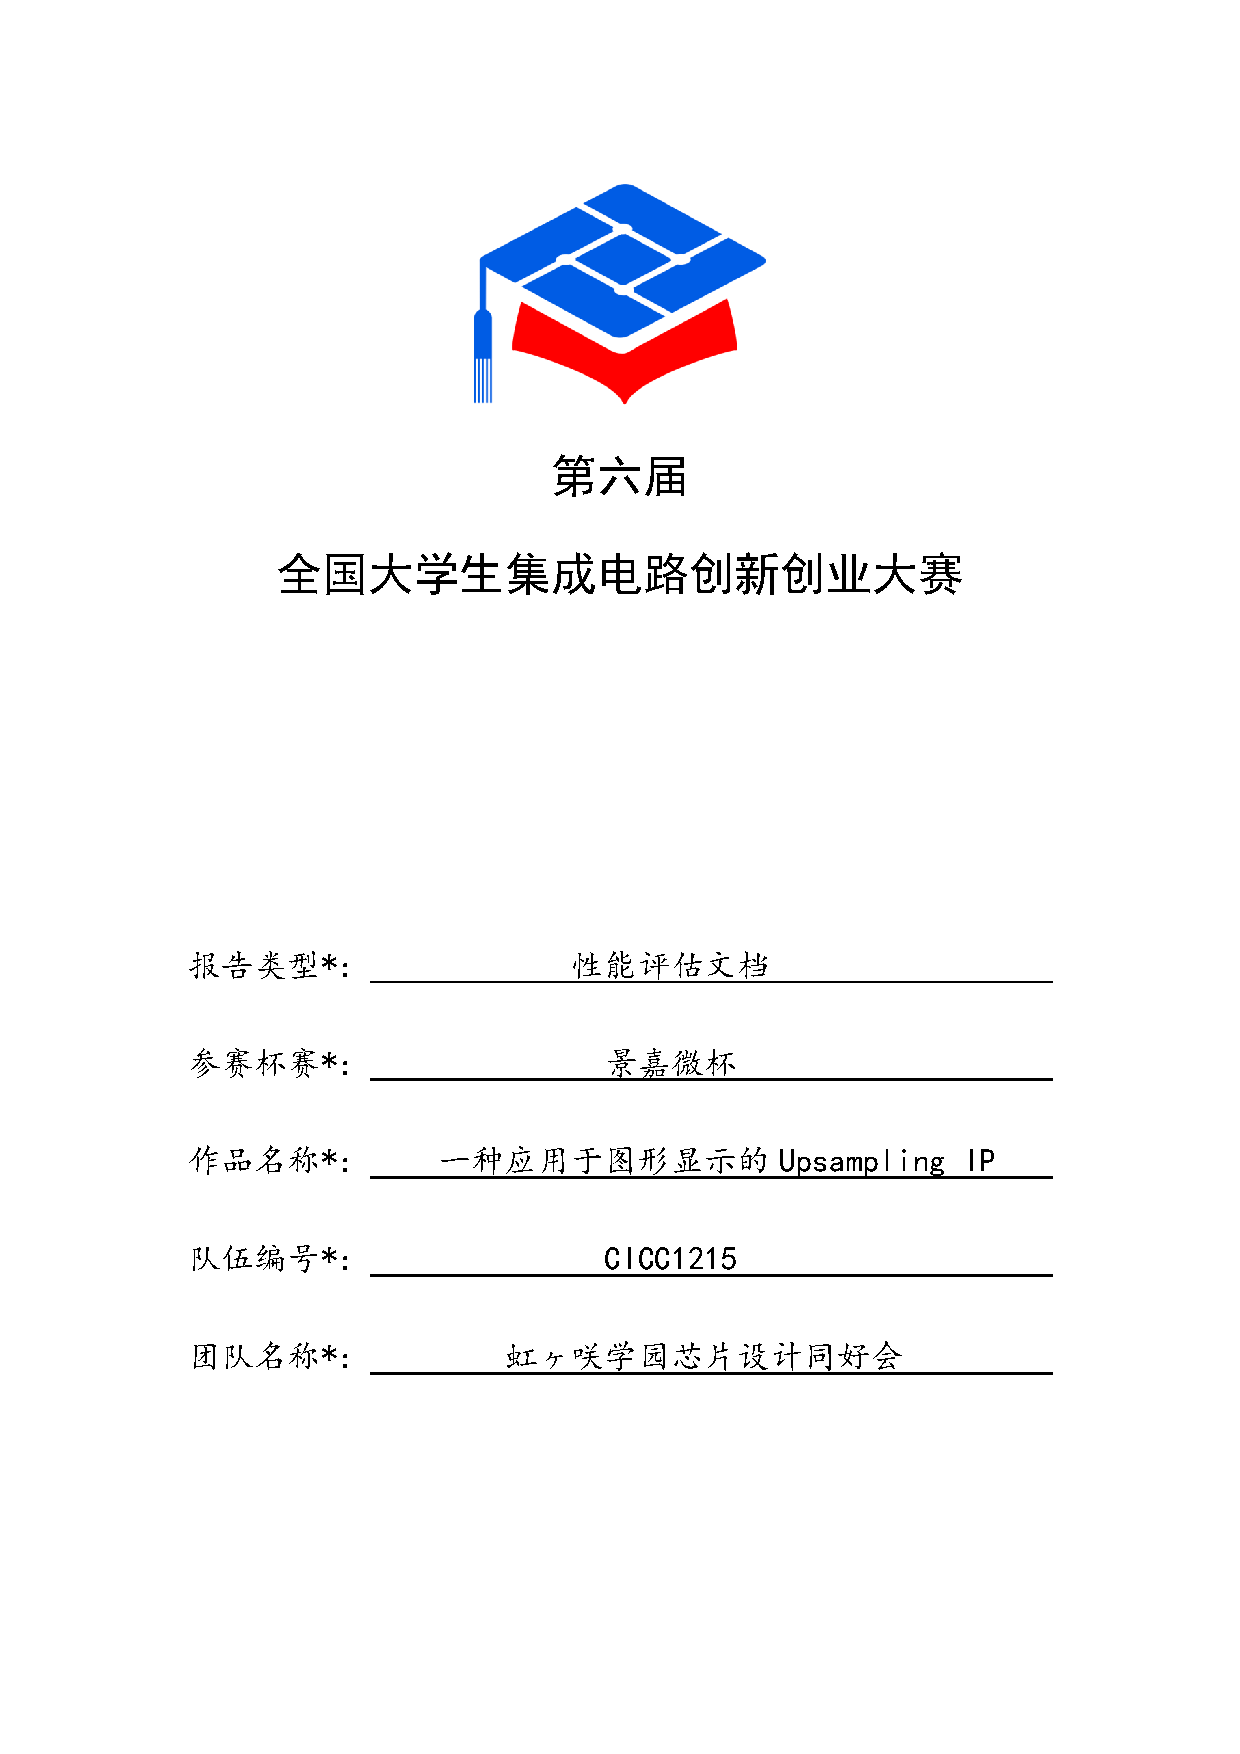
\includepdf{./pic/cover.pdf}
	\maketitle	
	\pagenumbering{Roman}
	\setcounter{page}{1}
	%-----------------------前言------------------
	\begin{center}
		\Huge\textbf{前言}
	\end{center}~\
	
	本文档(性能评估文档)仅作为虹ヶ咲学园芯片设计同好会(成员:黄金源、邓立唯、林明锋)参加第六届全国大学生集成电路创新创业大赛景嘉微杯赛初赛提交文档供评委评分使用。
	~\\
	\begin{flushright}
		\begin{tabular}{c}
			虹ヶ咲学园芯片设计同好会\\
			\today
		\end{tabular}
	\end{flushright}
	%-----------------------目录------------------
	\newpage
	\pagenumbering{Roman}	%Roman or arabic
	\setcounter{page}{1}
	\tableofcontents
	\newpage
	\setcounter{page}{1}
	\pagenumbering{arabic}
	
	%-----------------------正文----------------	
	\chapter{概述}
	性能评估主要分为三大部分,针对于每个设计 IP 进行单独评估分析,其中包括 Bicubic 上采样模块性能评估、纹理分类模块性能评估以及自适应锐化模块性能评估。
	
	\chapter{Bicubic 上采样模块性能评估}
	\section{性能参数}
	使用 Vivado 与 Synopsys Synplify Premier 进行时序分析。输入 $960\times540$ 图像数据作为基准。
		\subsection{最大频率}
			\begin{table}[h]
			\centering
				\begin{tabular}{|c|c|c|}
					\hline
					\textbf{FPGA Device Family} & \textbf{Analysis Tool}            & \textbf{Fmax (MHz)} \\ \hline
					Xilinx Virtex UltraScale+   & Synopsys Synplify Premier 2020.03 & 628.6               \\ \hline
					Xilinx Kintex UltraScale+   & Synopsys Synplify Premier 2020.03 & 417.2               \\ \hline
					\multirow{2}*{Xilinx Zynq UltraScale+}     & Synopsys Synplify Premier 2020.03 & 394.1               \\
					\cline{2-3}& Vivado 2021.1                     & 428.4               \\ \hline
					Xilinx Kintex 7             & Synopsys Synplify Premier 2020.03 & 361.7               \\ \hline
					Xinlinx Artix 7             & Synopsys Synplify Premier 2020.03 & 192.2               \\ \hline
					Intel Stratix 10            & Synopsys Synplify Premier 2020.03 & 260.7               \\ \hline
					Intel Max 10                & Synopsys Synplify Premier 2020.03 & 220.5               \\ \hline
					Intel Arria V               & Synopsys Synplify Premier 2020.03 & 142.5               \\ \hline
				\end{tabular}
			\end{table}
		\subsection{最大延迟}
		仅用于评估该IP的路径时延,不考虑受系统延迟或其他限制。假设图像输入宽为 $W$ 位像素。
		\begin{table}[h]
			\centering
			\begin{tabular}{|c|c|c|}
				\hline
				\textbf{描述}             & \textbf{时钟周期}                     & \textbf{Fmax (MHz)} \\ \hline
				Bicubic流水运算从输入到输出       & 13                                & 628.6               \\ \hline
				第一个像素进入到第一个像素输出         & $10\cdot W+28$                    & 417.2               \\ \hline
				最后一个像素进入到最后一个像素输出       & $13\cdot W + 31$                  & 394.1               \\ \hline
				Xilinx Zynq UltraScale+ & Vivado 2021.1                     & 428.4               \\ \hline
				Xilinx Kintex 7         & Synopsys Synplify Premier 2020.03 & 361.7               \\ \hline
				Xinlinx Artix 7         & Synopsys Synplify Premier 2020.03 & 192.2               \\ \hline
				Intel Stratix 10        & Synopsys Synplify Premier 2020.03 & 260.7               \\ \hline
				Intel Max 10            & Synopsys Synplify Premier 2020.03 & 220.5               \\ \hline
				Intel Arria V           & Synopsys Synplify Premier 2020.03 & 142.5               \\ \hline
			\end{tabular}
		\end{table}
		\subsection{吞吐量}
		用于评估不同图像帧大小进入。
		\begin{table}[h]
			\centering
			\begin{tabular}{|c|c|c|c|}
				\hline
				\textbf{输入分辨率} & \textbf{输出分辨率} & \textbf{吞吐量(FPS/MHz)} & \textbf{FPS@150MHz} \\ \hline
				320 x 240      & 1280 x 960     & 3.23                  & 484.7               \\ \hline
				480 x 270      & 1920 x 1080    & 1.92                  & 287.6               \\ \hline
				640 x 360      & 2560 x 1440    & 1.08                  & 162.1               \\ \hline
				960 x 540      & 3840 x 2160    & 0.48                  & 72.1                \\ \hline
			\end{tabular}
		\end{table}
	\section{资源使用量}
	Xilinx Zynq UltraScale+ 器件的资源利用结果是在 Vivado 综合器下,使用 DSP48E2 和 XPM 宏进行评估的。\par	
	% Please add the following required packages to your document preamble:
	% \usepackage{multirow}
	\begin{table}[h]
		\begin{tabular}{|c|cc|cccc|}
			\hline
			\multirow{2}{*}{\textbf{Device}} & \multicolumn{2}{c|}{\textbf{configuration}}                         & \multicolumn{4}{c|}{\textbf{Resource Utilization}}                                                                                            \\ \cline{2-7} 
			& \multicolumn{1}{c|}{\textbf{Input Resolution}} & \textbf{fCLK(MHz)} & \multicolumn{1}{c|}{\textbf{LUTS}} & \multicolumn{1}{c|}{\textbf{FFTs}} & \multicolumn{1}{c|}{\textbf{DSPs}}         & \textbf{BRAMs}         \\ \hline
			XCZU15EG                         & \multicolumn{1}{c|}{960 × 540}                 & 300                & \multicolumn{1}{c|}{431}           & \multicolumn{1}{c|}{694}           & \multicolumn{1}{c|}{49\textasciicircum{}1} & 2.5\textasciicircum{}3 \\ \hline
			XC7K325T                         & \multicolumn{1}{c|}{960 × 540}                 & 150                & \multicolumn{1}{c|}{1979}          & \multicolumn{1}{c|}{2713}          & \multicolumn{1}{c|}{30\textasciicircum{}2} & 2\textasciicircum{}3   \\ \hline
		\end{tabular}
	\end{table}
	其他器件的评估结果是使用 Verilog 自动推断完成的,可能由于每个器件的 DSP 模块的数据宽度不同而导致不同。实时视频 Bicubic IP 是为 Xilinx UltraScale+ 系列器件的 DSP48E2 模块特别优化的。为了最大限度地利用资源,建议使用这些器件进行合成。
	
	\chapter{纹理分类模块性能评估}
	由于该模块处于整合阶段,故未进行详细性能评估。
	\section{性能参数}
	使用 Vivado 进行时序分析。
		\subsection{最大频率}
		未进行评估。
		\subsection{最大延迟}
		仅用于评估该IP的路径时延,不考虑受系统延迟或其他限制。假设图像输入宽为 $W$ 位像素。
		\begin{table}[h]
			\centering
			\begin{tabular}{|c|c|}
				\hline
				\textbf{描述}       & \textbf{时钟周期}   \\ \hline
				高斯滤波运算从输入到输出      & 9               \\ \hline
				拉普拉斯滤波运算从输入到输出    & 4               \\ \hline
				纹理检测器运算从输入到输出     & 1               \\ \hline
				第一个像素进入到第一个像素输出   & $8\cdot W+14$   \\ \hline
				最后一个像素进入到最后一个像素输出 & $8\cdot W + 14$ \\ \hline
			\end{tabular}
		\end{table}
		\subsection{吞吐量}
		未进行评估。
	\section{资源使用量}
	Xilinx Zynq UltraScale+ 器件的资源利用结果是在 Vivado 综合器下,使用 DSP48E2 和 XPM 宏进行评估的。其他器件的评估结果是使用Verilog自动推断完成的,可能由于每个器件的 DSP 模块的数据宽度不同而导致不同。实时视频纹理分类 IP 是为 Xilinx UltraScale+ 系列器件的 DSP48E2 模块特别优化的。为了最大限度地利用资源,建议使用这些器件进行合成。\par 未进行评估。
	
	
	\chapter{自适应锐化模块性能评估}
	\section{性能参数}
	使用 Vivado 进行时序分析。
		\subsection{最大频率}
		此模块最大频率限制是由于内部设计使用了 URAM288,其最大速率由工艺决定。
		\begin{table}[h]
			\centering
			\begin{tabular}{|c|c|c|}
				\hline
				\textbf{FPGA Device Family}  & \textbf{Analysis Tool} & \textbf{Fmax (MHz)} \\ \hline
				Xilinx Virtex UltraScale+    & Vivado 2021.2          & 355.1               \\ \hline
				Xilinx Kintex UltraScale+    & Vivado 2021.2          & 351.3               \\ \hline
				Xilinx Zynq UltraScale+      & Vivado 2021.2          & 344.4               \\ \hline
				Xilinx Versal AI Core Series & Vivado 2021.2          & 348.8               \\ \hline
			\end{tabular}
		\end{table}	
		\subsection{最大延迟}
		仅用于评估该IP的路径时延,不考虑受系统延迟或其他限制。假设图像输入宽为 $W$ 位像素。
		\begin{table}[h]
			\centering
			\begin{tabular}{|c|c|c|}
				\hline
				\textbf{描述}       & \textbf{时钟周期}   & \textbf{Fmax (MHz)} \\ \hline
				锐化卷积运算从输入到输出      & 10              & 355.1               \\ \hline
				第一个像素进入到第一个像素输出   & $3\cdot W+10$   & 351.3               \\ \hline
				最后一个像素进入到最后一个像素输出 & $3\cdot W + 10$ & 344.4               \\ \hline
			\end{tabular}
		\end{table}
		\subsection{吞吐量}
		未进行评估。
	\section{资源使用量}	
	Xilinx Zynq UltraScale+ 器件的资源利用结果是在 Vivado 综合器下,使用 DSP48E2 和 XPM 宏进行评估的。其他器件的评估结果是使用 Verilog 自动推断完成的,可能由于每个器件的 DSP 模块的数据宽度不同而导致不同。实时视频自适应锐化 IP 是为 Xilinx UltraScale+ 系列器件的 DSP48E2 模块特别优化的。为了最大限度地利用资源,建议使用这些器件进行合成。
	\begin{table}[h]
		\centering
		\begin{tabular}{|c|cc|ccccc|}
			\hline
			\multirow{2}{*}{\textbf{Device}} & \multicolumn{2}{c|}{\textbf{Configuration Parameter}}               & \multicolumn{5}{c|}{\textbf{resource utilization}}                                                                                                               \\ \cline{2-8} 
			& \multicolumn{1}{c|}{\textbf{Input resolution}} & \textbf{fclk(MHz)} & \multicolumn{1}{c|}{\textbf{LUTs}} & \multicolumn{1}{c|}{\textbf{FFs}} & \multicolumn{1}{c|}{\textbf{DSPs}} & \multicolumn{1}{c|}{\textbf{BRAM}} & \textbf{URAM} \\ \hline
			XC2V15EG                         & \multicolumn{1}{c|}{960 × 540}                 & 300                & \multicolumn{1}{c|}{228}           & \multicolumn{1}{c|}{1633}         & \multicolumn{1}{c|}{148}           & \multicolumn{1}{c|}{5}             & 10            \\ \hline
		\end{tabular}
	\end{table}
	

\end{document}
